\documentclass{article}
\usepackage{graphicx}
\usepackage[margin=1in]{geometry}
\usepackage{multicol}


\title{ORIE 4741 Final Project Report}
\author{Aparna Calambur (ac987), Jack Schluger (jes543), Wanxing Lu (wl473)}
\date{December 13, 2020}

\begin{document}
\twocolumn
\maketitle

\section{Introduction}
In our final project, we built a predictive model to determine the ideal price point of a domestic US flight traveling from point A to point B. Our goal was to develop a model that can be used from the perspective of an Airline company to determine the ideal price of airplane tickets to maximize profit while staying competitive in the market given the competition. Moreover, we hope that our findings not only help airlines price future flights, but also help consumers decide when and where to fly to maximize a trip within their budget.\\\\
Though air travel may not be a mode of transportation that an individual considers on a daily basis, nevertheless, it inexplicably affects how people are connected and communicate across the nation. On a personal and current perspective, air travel and price tickets also determine when were are able to visit our families, return back to school, and travel across the country. From an economic standpoint, the airline industry constitutes a significant force within the U.S. economy: according to the FAA, ?Aviation accounts for more than 5\% of our Gross Domestic Product.?$^{[1]}$ As an industry that many people rely on for work and personal means, domestic flights impact many people?s lives every day. Therefore, it is a vital task to understand how prices function within this industry: both to improve efficiency for these far reaching airlines and to help consumers understand pricing within the domestic flight market.\\\\
From thorough analysis of historical plane ticket data as well as fitting multiple models to the processed data, we believe that our project can provide accurate predictions that can help both the airline industry and the individual consumer alike. Through an iterative design process, we discover two model architectures that effectively model this problem space and will allow both consumers and airlines to understand historical and future trends in domestic flight pricing. 


\section{Datasets}
\subsection{Exploring the data}

Our project analyzes the dataset from the US Department of Transportation?s Domestic Airline Consumer Airfare Report from 2019$^{[2]}$. This dataset contains 213175 rows and 23 columns describing information for airport pair markets. Each row contains an origin airport and city, destination airport and city, year, time of year (quarter), average fare, average fare for the carrier with the largest market share, average fare for the lowest carrier, number of miles, passengers per day, and geocoded information.

\subsection{Data Cleaning}
After cleaning and pre-processing, our resulting dataset contains 201392 rows and 24 columns.\\\\
We create an additional row to the original 23 rows by constructing a ?when? column that combines the columns year with the financial quarter via the following formula: $when = year + (quarter - 1)/4$. \\\\
Of the 213175 original rows, 201392 rows have complete data without any missing values and we do not have any corrupted values. Since a significant majority of our data is complete, we decided to remove the rows with missing values rather than impute them. We have over 200,000 rows with complete data which maintains 95\% of the original data. Additionally, the rows with missing data included outlier flights from smaller towns or airlines where we cannot accurately impute the missing values from the rest of the data. These flights are priced very different compared to typical airlines and may not be helpful to our overall analysis.

 \begin{figure}[h]
\centering
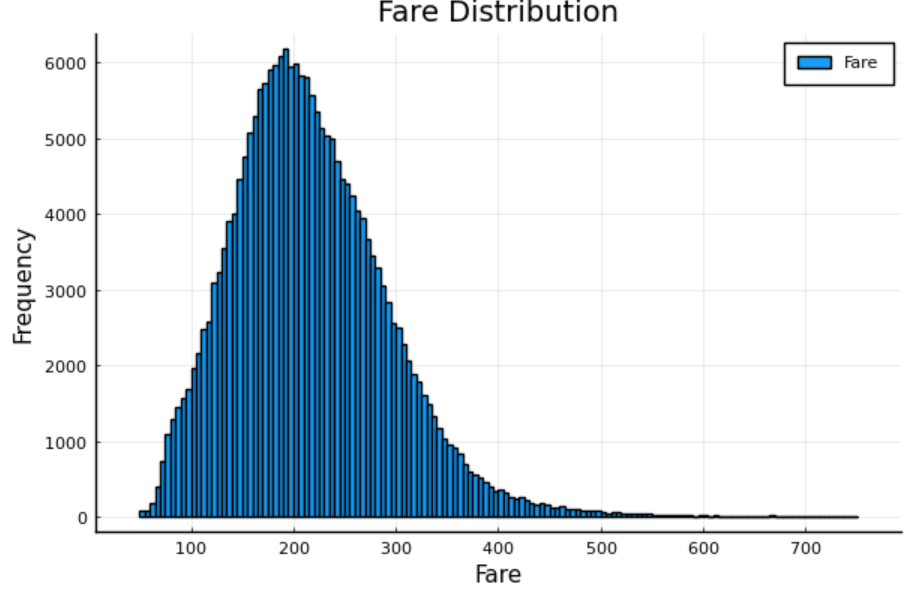
\includegraphics[scale=.5]{images/hist_plot.png}
\caption{Fare Histogram}
\end{figure}

\begin{figure*}[h]
\centering
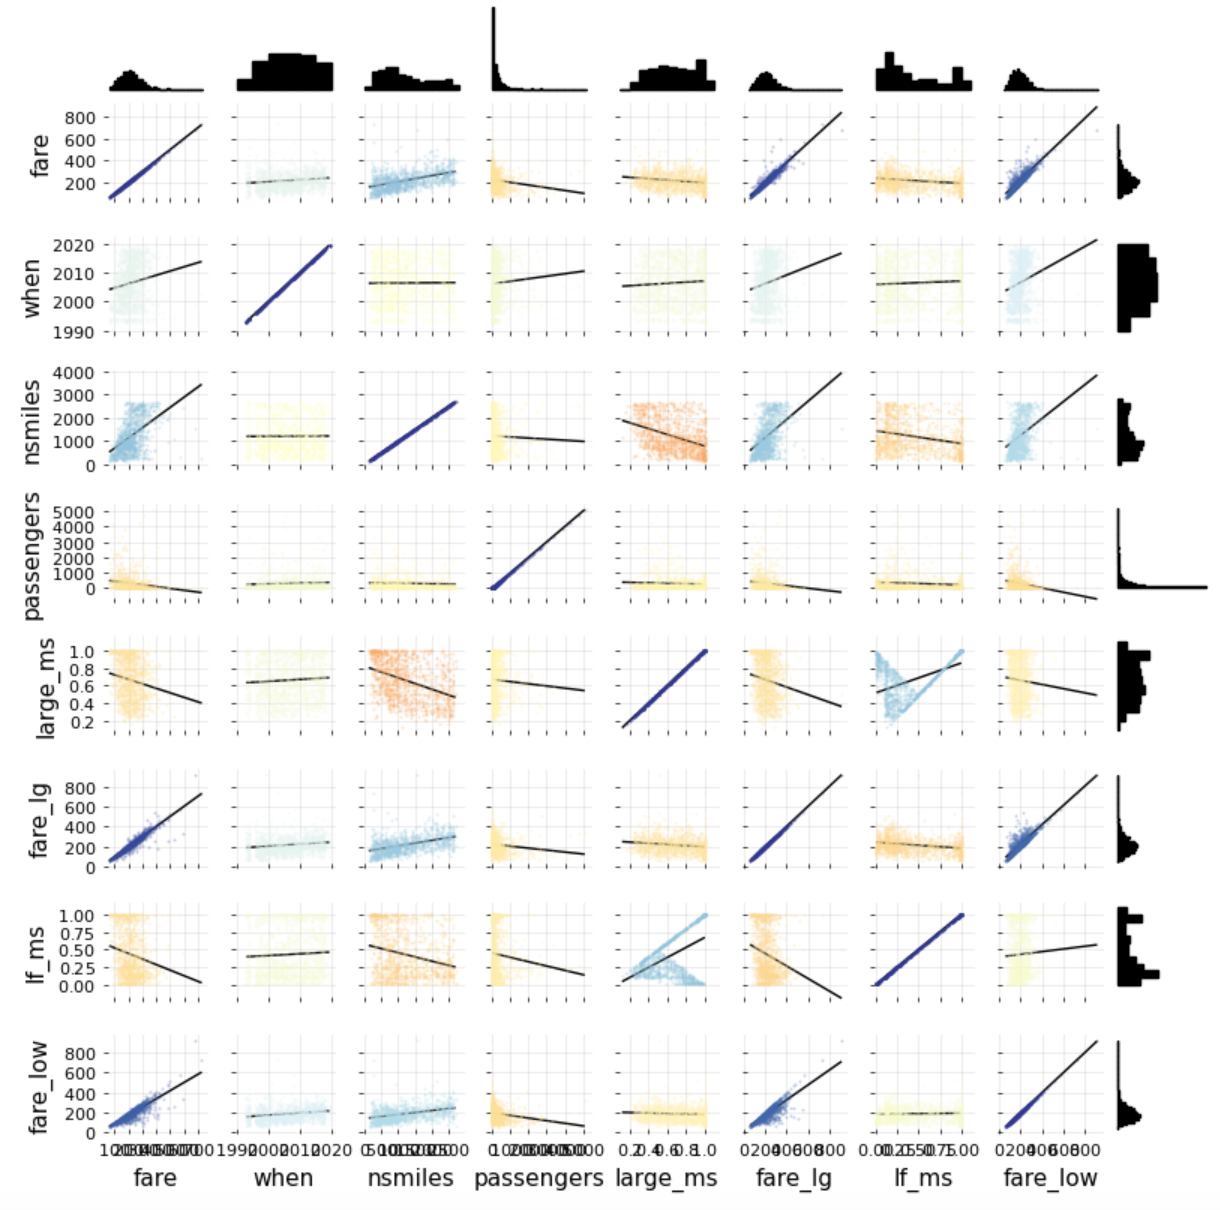
\includegraphics[scale=.4]{images/corr_plot.png}
\caption{Correlation Plot}
\end{figure*}

\subsection{Data Visualizations}

In this section we highlight some useful plots to help us better understand the data. Figure 1 shows a histogram of average fares. Each data point is an average fare across all flights from a given city to another, in one quarter of a given year, and the histogram shows the frequency of different average fares. From initial observation, most prices fall between \$100 to \$400. Moreover, the average fare statistic has mean 217.7, median 208.4, and standard deviation 82.6. We excluded large outliers before constructing the plot, which would otherwise have a long, sparse tail, and yet this histogram is slightly right skewed with a handful of very expensive tickets. This plot allows us to understand what is a normal range of ticket prices and what we should expect in our predictions. \\\\
Figure 2 shows us the correlation matrix plot of all numerical variables against one another. This plot gives us a better understanding of how the variables correlate with our target and each other; blue indicates a positive correlation while orange indicates a negative correlation. The darker the color, the stronger the correlation. We can see that the variables  when, nsmiles, fare\_lg, and fare\_low all have positive relationships with fare. Intuitively, all of these relationships make sense. As the when variable increases, fare increases because of inflation: ticket prices have gone up over the years. It also makes sense that as nsmiles increase so does fare because nsmiles represents number of miles: flights that travel further cost more. The variables fare\_lg and fare\_low represents the average fare for the air carrier with the largest market share and lowest respectively. Both variables are already related to fare. As average fares for specific carriers increase, so should the fare for any specific flight.\\\\ Meanwhile, passengers, large\_ms, and lf\_ms all have a negative correlation with fare. We can also make sense of these relationships as well. As the number of passengers increase, fare decreases because these are likely large flights that are less exclusive and so they would be cheaper. The variables large\_ms and lf\_ms represent market share for the carrier with highest market share and marketshare for the carrier with the lowest fare, respectively. As market share increases, it makes sense for fare to drop because those are likely big companies that the average US traveler uses, so fares would be less because they aren't as exclusive. \\\\
In general, there are no strong relationships between the other variables and each other except for: nsmiles and large\_ms which has a negative relationship, nsmiles and lf\_ms which has a negative relationship, large\_ms and lf\_ms is positive, fare\_low and fare\_lg is positive, and fare\_lg and lf\_ms is negative.


\section{Methods}

\subsection{Feature Engineering}

Our data was compiled of both numerical and nominal data types. We used one-hot encoding on our nominal data before using it to train and test our model. The motivation behind one-hot encoding is that it allows us to use an indicator function to turn each category into a boolean value. \\\\
Once we computed the one-hot vectors for each nominal feature, we combined that with the numerical data before training our model. 
\subsection{Feature Selection}
We started with 24 columns in our original dataset:
["tbl", "Year", "quarter", "citymarketid\_1", "citymarketid\_2", "city1", "city2", 
"airportid\_1", "airportid\_2", "airport\_1", "airport\_2", "nsmiles", "passengers", 
"fare", "carrier\_lg", "large\_ms", "fare\_lg", "carrier\_low", "lf\_ms", "fare\_low",
"Geocoded\_City1", 
\\"Geocoded\_City2", "tbl1apk", "when"]
\subsubsection{Dropping Features}
We dropped some redundant or irrelevant columns at the start. The columns ["tbl", "tbl1apk?] held information on the table name from the database which is irrelevant to our task. ["Year", "quarter"] were already consolidated into the when column, as described in section 2.2. ["city1", "city2", "Geocoded\_City1", "Geocoded\_City2"] represent the names and geo-coded location of the origin and destination cities. This information is already captured by the id?s of the cities in the columns citymarketid\_1 and citymarketid\_2. ["airport\_1", "airport\_2"] encode the names of the origin and destination airports. This information is already captured by the id?s of the airports in the columns airportid\_1 and airportid\_2
\\\\
In the end, we are left with these 14 to use for our model: ["citymarketid\_1", "citymarketid\_2", "airportid\_1", "airportid\_2", "nsmiles", "passengers", "fare", "carrier\_lg", "large\_ms", "fare\_lg", "carrier\_low", 
\\"lf\_ms", "fare\_low", "when"].

\subsubsection{Feature Sets}
We had several different feature sets that we created to train our model on. We experimented with both the number of features included and how we pre-processed those features. Specifically, we explored treating the city and airport id?s as both numerical and nominal data. The id's for all of these columns are integers, but they are not continuous since they represent discrete cities and airports. We wanted to experiment with the trade-off of using them as numerical vs. nominal to see its impact on the accuracy of our model. In total we trained our model on 4 different sets of features to predict fare. 


\paragraph{Feature Set 0:}
\\Table 1 shows our simple baseline set of features using domain knowledge. We chose these features because they were the most basic information needed to predict the price of a flight.
\begin{table}[h!]
\centering
\begin{tabular}{ |p{3cm}||p{3cm}|  }
 \hline
 \multicolumn{2}{|c|}{Feature Set 0} \\
 \hline Feature & Type\\
 \hline
airportid\_1 & Int64 \\ 
airportid\_2 & Int64 \\
when & Float64 \\
 \hline
\end{tabular}
\caption{Feature Set 0 Table}
\label{table:1}
\end{table}
\paragraph{Feature Set 1:}
This next feature set can be seen in table 2. It only uses numerical data and treats the airport and city id's as numerical. We wanted to be able to compare these results with the results including nominal data to see whether nominal data is helpful in improving accuracy.
\begin{table}[h!]
\centering
\begin{tabular}{ |p{3cm}||p{3cm}|  }
 \hline
 \multicolumn{2}{|c|}{Feature Set 1} \\
 \hline Feature & Type\\
 \hline
 citymarketid\_1 & Int64\\
 citymarketid\_2 & Int64\\
airportid\_1 & Int64\\
airportid\_2 & Int64\\
nsmiles & Int64\\
passengers & Int64 \\
large\_ms & Float64 \\
fare\_lg & Float64\\
lf\_ms & Float64\\
fare\_low & Float64\\
when & Float64\\
 \hline
\end{tabular}
\caption{Feature Set 1 Table}
\label{table:1}
\end{table}
\paragraph{Feature Set 2:} This feature set is in table 3. We include all of the columns, both numerical and nominal. We continue to treat the city and airport id's as numerical. Including all features allows us to compare to our previous models that use a smaller feature set to see if nominal data adds value. 

\paragraph{Feature Set 3:} Finally, this feature set is also in table 3. We include all of the columns, treating the city and airport id's as nominal data. We aim to see how our model performs treating city and airport id's as nominal and numerical, in order to compare performance. 
\begin{table}[h!]
\centering
\begin{tabular}{ |p{3cm}||p{3cm}|  }
 \hline
 \multicolumn{2}{|c|}{Feature Sets 2 and 3} \\
 \hline Feature & Type\\
 \hline
 citymarketid\_1 & Int64\\
 citymarketid\_2 & Int64\\
airportid\_1 & Int64\\
airportid\_2 & Int64\\
nsmiles & Int64\\
passengers & Int64 \\
carrier\_lg & String\\
large\_ms & Float64 \\
fare\_lg & Float64\\
carrier\_low & String\\
lf\_ms & Float64\\
fare\_low & Float64\\
when & Float64\\
 \hline
\end{tabular}
\caption{Feature Sets 2 and 3 Table}
\label{table:1}
\end{table}
\subsection{Baseline Model}
The first preliminary analysis we ran was a simple linear model to predict fare given a source airport, a destination airport, and when the flight is. We used the Julia backslash operator to solve the least squares problem to predict the fare given these features and a bias, using 80\% of the dataset for training and holding out 20\% of the data for validation.\\\\
In this experiment, we observed a root mean squared error (RMSE) of 82.0 on the training set, and 81.1 on the held out validation set. This indicates that this simple linear model is not overfitting, and we can add complexity to our model in the next round of modeling. Further, this is an encouraging result because this error is about the same as the standard deviation of the average fare statistic, which is 82.6. 
\subsection{Advanced Regression Methods}
After building a simple least squares model, we decided to pursue a stronger methodical approach for model selection. 
\subsubsection{Two Goals}
Following a two pronged method of analyzing models for interpolation and extrapolation, we report a two dimensional analysis: selecting models based on extrapolation or interpolation validation performance, and reporting final extrapolation and interpolation test performance of all selected models.
\subsubsection{Modeling}
We sought out to improve upon our current simple linear regression model, so we decided to use different regression models to predict fare, experimenting with regularization and loss. Our main methods included ridge regression, lasso regression, and quantile regression.\\\\
For our regression models, the loss functions we used included: L1, quadratic, and quantile. These are all loss functions for predicting real-valued data. In this case we are predicting price, which is real-valued. We also experimented with common regularization methods for predicting real-valued data including: lasso, ridge, non-negative constraint, and no regularization. 
\subsubsection{Hyperparameter Tuning}
In addition to experimenting with regularization, loss functions, and feature subsets, we did hyperparameter tuning for each model, including setting alpha values for quantile loss, learning rate, and the lambda value for regularization.\\\\
In total we trained 640 models each to select the best model for interpolation and extrapolation. 
\begin{table*}[h!]
\begin{center}
\def\arraystretch{2} % 1 is the default, change whatever you need
\begin{tabular}{ |c|c|c|c| } 
 \hline
 Architecture Name & Featurization & Optimization Objective & Learning Rate \\ 
 \hline
I0 & 0 & 
$\frac{1}{n}\sum_{i=1}^n(y_i - w^Tx_i)^2+\frac{3}{4}\sum_{i=1}^d w_i^2$ 
&  0.1 \\
I1 & 1 & 
$\frac{1}{n}\sum_{i=1}^n(y_i - w^Tx_i)^2$
&  0.7 \\
I2 & 2 & 
$\frac{1}{n}\sum_{i=1}^n(y_i - w^Tx_i)^2+\frac{1}{2}\sum_{i=1}^d w_i^2$
&  0.3 \\
I3 & 3 & 
$\frac{1}{n}\sum_{i=1}^n(y_i - w^Tx_i)^2+\frac{3}{4}\sum_{i=1}^d w_i^2$
&  0.7 \\
 \hline
\end{tabular}
\end{center}
\caption{Architecture of models selected based on interpolation performance}
% \label{table:}
\end{table*}

\begin{table*}[h!]
\begin{center}
\def\arraystretch{2}%  1 is the default, change whatever you need
\begin{tabular}{ |c|c|c|c| } 
 \hline
 Architecture Name & Featurization & Optimization Objective & Learning Rate \\ 
 \hline
E0 & 0 &  
$\frac{1}{n}\sum_{i=1}^n\frac{3}{4}(y_i - w^Tx_i)_+ + \frac{1}{4}(y_i - w^Tx_i)_-$ 
&  0.7 \\
E1 & 1 &  
$\frac{1}{n}\sum_{i=1}^n\frac{3}{4}(y_i - w^Tx_i)_+ + \frac{1}{4}(y_i - w^Tx_i)_-$ 
&  0.1  \\
E2 & 2 & 
$\frac{1}{n}\sum_{i=1}^n\frac{3}{4}(y_i - w^Tx_i)_+ + \frac{1}{4}(y_i - w^Tx_i)_-$ 
&  0.1  \\
E3 & 3 & 
$\frac{1}{n}\sum_{i=1}^n\frac{3}{4}(y_i - w^Tx_i)_+ + \frac{1}{4}(y_i - w^Tx_i)_-$ 
&  0.3  \\
 \hline
\end{tabular}
\end{center}
\caption{Architecture of models selected based on extrapolation performance}
% \label{table:}
\end{table*}


\subsection{Models for Interpolation}
To select our first set of models, we optimized for interpolation. First we divided our dataset into a train and test set by randomly holding out 15\% of the dataset for the test set. Then, we trained all our candidate architectures using 15-fold cross validation on this training set to find the best performing models in terms of Mean Squared Error.\\\\
This procedure selects models based on how well they can do interpolation with respect to time because randomly choosing data points for the train and validation sets on each fold means these data points are from the same distribution as the train set. Moreover, we maintain a held out test set that is also from the same distribution.\\\\
We report results from the best performing model architecture for each feature set; the models selected for interpolation are reported in Table 4.

\subsection{Models for Extrapolation}

To select our second set of models, we optimized for extrapolation. First we divided out dataset into train, and test sets according to time: we used all data points from during or after 2015 as the test set, and used the rest of the data for training and model selection. We further divided this training data into a train set of all data points from before the first quarter of 2011, and a validation set of all data points from during or after the first quarter of 2011. These dates were chosen to produce a 70\% / 30\% / 30\% train / validation  / test set split. Then, we trained all our candidate architectures on the train set and used the validation set to perform model selection.\\\\
This procedure selects models based on how well they can do extrapolation with respect to time because the validation set contains data that is entirely in the future of the train set. Moreover, the held out test set contains data that is strictly in the future of the train and validation sets as well.\\\\
We report results from the best performing model architecture for each feature set; the models selected for extrapolation are reported in Table 5.

\begin{table*}[h!]
\begin{center}
\begin{tabular}{ |c|c|c| } 
 \hline
 Model Name & Interpolation RMSE & Extrapolation RMSE \\ 
 \hline
I0 & 81.55 & 78.80 \\
I1 & 79.92 & 77.40 \\
I2 & 80.02 & 77.50 \\
\textbf{I3} & \textbf{52.74} & \textbf{48.97} \\
 \hline
\end{tabular}
\end{center}
\caption{Performance of models selected for interpolation  performance during validation}
% \label{table:}
\end{table*}

\begin{table*}[h!]
\begin{center}
\begin{tabular}{ |c|c|c| } 
 \hline
 Model Name & Interpolation RMSE & Extrapolation RMSE \\ 
 \hline
E0 & 93.85 & 73.32 \\
E1 & 91.14 & 71.51 \\
E2 & 91.14 & 71.51 \\
\textbf{E3} & \textbf{18.76} & \textbf{44.33} \\
 \hline
\end{tabular}
\end{center}
\caption{Results on models selected for extrapolation performance during validation}
% \label{table:}
\end{table*}

\section{Results} 
\subsection{Interpolation Metric}
For \textit{every} model selected to be included in the final evaluation, we retrain the model architecture on the entire interpolation train set, and report its mean squared error on the held out interpolation test set. See section 3.5 for a description of these sets. 

\subsection{Extrapolation Metric}
For \textit{every} model selected to be included in the final evaluation, we retrain the model architecture on the entire extrapolation train set and validation sets (all data before 2015) and report its mean squared error on the held out extrapolation test set (all data during or after 2015). See section 3.6 for a description of these sets. 

\subsection{Findings}
In table 4 we describe the architecture and hyperparameters of the best performing model architectures based on interpolation performance; in table 6, we show the interpolation and extrapolation performance of these models on held out data. Similarly, in table 5 we describe the architecture and hyperparameters of the best performing model architectures based on extrapolation performance; in table 7, we show the interpolation and extrapolation performance of these models on held out data. \\\\
These results show that feature set three is the most informative, achieving the lowest MSE on both extrapolation and interpolation metrics. Further, for all feature sets we tried, quadratic loss is the best model for interpolation and quantile loss on the 0.75 quantile is the best model for extrapolation. The best models for extrapolation on all feature sets do not contain regularization, whereas for interpolation the best models for all feature sets (other than number one) included some quadratic regularization. \\\\
Finally, these results show a clear benefit to tailoring model architecture selection based on knowledge of how a model will be used. Our best extrapolation-optimization-selected architecture (E3) significantly outperforms any interpolation-optimization-selected architecture on the extrapolation metric, despite the fact that all models architectures are retrained on the same dataset to report extrapolation performance. Similarly, our best interpolation-optimization-selected architecture (I3) significantly outperforms any extrapolation-optimization-selected architecture on the interpolation metric, despite the fact that all model architectures are retrained on the same dataset to report interpolation performance.

\section{Error Analysis}
We perform an error analysis on the best model in terms of the interpolation metric (I3) and the best model in terms of the extrapolation metric (E3). In Figure 3 we show the distribution of errors I3 makes on the interpolation metric, and in Figure 4 we show the distribution of errors E3 makes on the extrapolation metric. These histograms have a long tail with very low frequencies, which we truncate for ease of visualization. We also included a red line to indicate the standard deviation of the prices.\\\\
Based on these histograms, we see that in both cases the vast majority of errors are small?with high probability, our models will predict a price that is close to the correct price. In both graphs, we observe that the respective model achieves a root squared error of less 82.6, the standard deviation of the overall price distribution (see section 2.3), on a clear and overwhelming majority of examples. Therefore, we conclude that while our models are not perfect, we should be confident in model I3 for modeling historical prices, and we should be confident in model E3 for modeling future prices (if we expect future prices to align with past trends; this may not be currently true with the ongoing covid pandemic as the resulting global aviation shifts are not represented in this dataset).   

\begin{figure}[h]
\centering
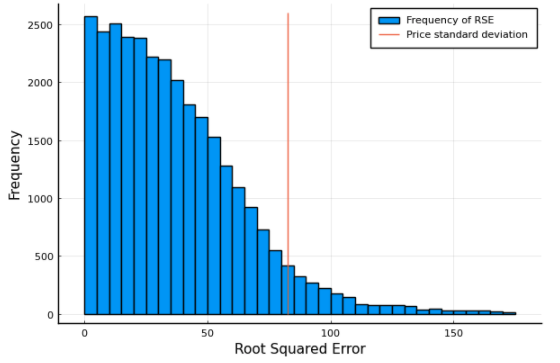
\includegraphics[scale=.40]{images/I3_Ierrors.png}
\caption{Histogram of Errors model I3 makes on the interpolation metric}
\end{figure}

\begin{figure}[h]
\centering
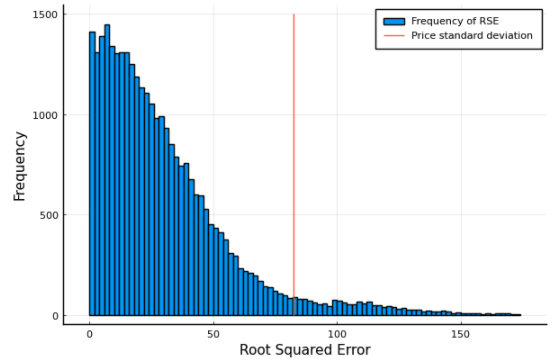
\includegraphics[scale=.40]{images/E3_Eerrors.png}
\caption{Histogram of Errors model E3 makes on the extrapolation metric}
\end{figure}

\section{Application}
Given the historical data that our models trained and evaluated on, we believe that our model creates an accurate prediction for future prices. However, the conditions of the recent and ongoing pandemic has had a subsequent effect in domestic travel, and thus these predictions may not be accurate for the current situation or years in the near future.\\\\
However there are still some patterns that remain proportionally unaffected by the pandemic; for example, there still is a peak in travel demand in the winter season due to the winter holiday breaks. Thus, we still believe that our data and analysis will be beneficial for companies to analyze to adjust their prices, while also factoring the effect of the pandemic on the general prices. In other words, our analysis provides a generalization of the trends of optimal prices, which can then be taken into consideration for current and future pricing.\\\\
In addition, we believe that having our model released as public information will not only help the airline companies, but also the consumers. They will be able to understand the trends of fluctuating airline tickets better to help plan their flying itineraries and budgets for traveling. The weight of public knowledge can also prevent airline tickets from raising their prices unreasonably and without bound, at the expense of the consumers.

\section{Weapons of "Math" Destruction}
%Lecture https://people.orie.cornell.edu/mru8/orie4741/lectures/limits.pdf
The definition of a weapon of math destruction is a predictive model whose outcome is not easily measurable, whose predictions can have negative consequences, or that creates self-fulfilling (or defeating) feedback loops.\\\\
None of our models are  weapons of math destruction, because they do not radically change what any actor in the flight market can do. While our models can allow anyone to understand the past ebbs and flows of the domestic flight market, or allow anyone to estimate flight prices in the future, our these models are not weapons of math destruction because of the limited ways this information can be used.\\\\
First, the outcome of our models is easily measurable: the models predict a concrete price given a data and endpoints for a trip. Moreover, these prices can be easily compared to real prices as real flights are scheduled and tickets are made available to consumers.\\\\
Next, our predictions may cause some small negative consequences, but they do not have systematic negative consequences that would render our models weapons of math destruction. Small negative consequences may include airlines making slightly less profits if consumers can more effectively choose flights within their budget. However, we think large negative consequences are not at play because flying generally is so expensive and traveling is so time consuming that while our models may help individuals optimize their interactions with the flight market (as a consumer or airline), they will not significantly change their behavior. This model can facilitate some changes in behavior, but not radical enough changes such as changing a decision to fly vs. not to fly that there will be large negative consequences because people already have personal and professional frameworks established for making these more impactful decisions. \\\\
Finally, our models do not create self-fulfilling or self-defeating feedback loops, because regardless of what our model predicts, consumers are still bound by the will of airlines with regard to when and where they fly, and how much they pay for their tickets. Because flights are not purchased via bidding but rather at a set price, our model will not immediately create a feedback loop on flight prices because consumers have little way to convey their desired price to airlines. Moreover, airlines are not likely to change prices based on response to demand induced or shifted as a consequence of our models' information, because airlines always try to have completely full flights and thus can easily miss increased demand for a particular flight. 


\section{Fairness}
%Lecture https://people.orie.cornell.edu/mru8/orie4741/lectures/fairness.pdf
We believe that fairness is not a key criterion for evaluating our models. The information and historical data that we gather to construct and train our model is not targeted to a specific group of people. Moreover, the numbers are quantitative and objective and does not reflect the biases of media sources such as the news.\\\\
Though it is likely that the prices of flights will continuously rise over the succeeding years, that is a common trend within any capitalistic good with an uncapped market. However, our model will not cause the prices of flights to increase without limit because the outputs are still bounded by demand and the prices the general public can afford. In fact, since airline companies may be incentivized to increase their prices to maximize profits at the expense of their consumers, our model provides transparency of pricing. Thus, our model will help consumers regain buying power and prevent airlines from raising prices more than what the consumers are willing to pay by facilitating more informed decisions for consumers. 

\section{Future Work}
In the future, we want to continue incorporate recent data into our models since the pandemic has largely affected the demand and flight prices that is unprecedented by previous years. In addition, our current data is gathered in quarterly periods and moving forward, we would like to improve the accuracy of our predictions by extrapolating data with more fine grain time intervals, such as monthly or weekly data points.\\\\
Additionally, we trained a total of 1280 models for this analysis, but we still have more models to explore. In our current method, we experimented with regression models to predict the price points such as linear regression, ridge, lasso, and quantile. In the future we would like to experiment with nonlinear methods such as Neural Networks, Boosted Random Forest, and advanced linear methods such as Principal Components Regression. Some of these methods are outside of the scope of this class, but it would be interesting to compare how the models created by those methods would perform in comparison to our models.
\newpage

\section{Bibliography}
\begin{enumerate}
    \item Federal Aviation Administration. (2016, November). The Economic Impact of Civil Aviation on the U.S. Economy.
    \item U.S. Department of Transportation. (2019, November). Consumer Airfare Report: Table 1a - All U.S. Airport Pair Markets.
\end{enumerate}

\end{document}